\section{Evaluation}
\label{sec:evaluation}

In this section, we quantify the benefits of using a crowd-shared WMN for public Internet access. In Section \ref{evaluation:environment}, we present the simulation environment, the modeling of router on/off periods, and the metrics used to evaluate the WMN efficiency. Section \ref{evaluation:results} provides a comparative study between a crowd-shared network, such as PAWS, and a WMN based on our simulation results.

\subsection{Simulation Environment}
\label{evaluation:environment}

%Using python, we developed a discrete event simulator to model the behavior of guest flows in a crowd-shared network connected through a wireless mesh network. We use the TFA wireless mesh topology \cite{}, that consist of 21 nodes to model a network of access home routers. Each router possesses an Internet connection from which it provides potential guests with a maximum of 8 Mbps in upload direction. In addition, the nodes are interconnected using an 802.11ac wireless mesh network with a capacity of 200 Mbps.

We developed a simulator that models the behavior of data flows that are generated by guest users in a crowd-shared WMN. We use the TFA wireless mesh topology \cite{TFA} which consists of 21 nodes (Fig. \ref{fig:topology}). Each node in this figure represents a home router with shared Internet access bandwidth, whereas each edge is a wireless mesh link. Guest user flows arrive randomly at different home routers. Each generated flow has a rate and lifetime sampled out of a uniform and an exponential distribution, respectively. The guest user flows arrive to the network according to a Poisson process.

We model the availability of the home access routers using an on-off Markov chain. On and off times are exponentially distributed with mean values $\mu_{on = 106}$ minutes and $\mu_{off} = 555$ minutes. We parameterize the exponential distributions using datasets from the PAWS deployment in UK. Fig. \ref{fig:active_routers} shows the number of active routers along 60 hours of simulation. We can see that out of 21 routers less than 12 routers are simultaneously available.

%To reflect real world traffic, we consider guest flows that arrive to the network according to a Poisson process. Each flow has a constant bit rate which is sampled out of a uniform distribution.

\begin{figure}[t]
\begin{center}
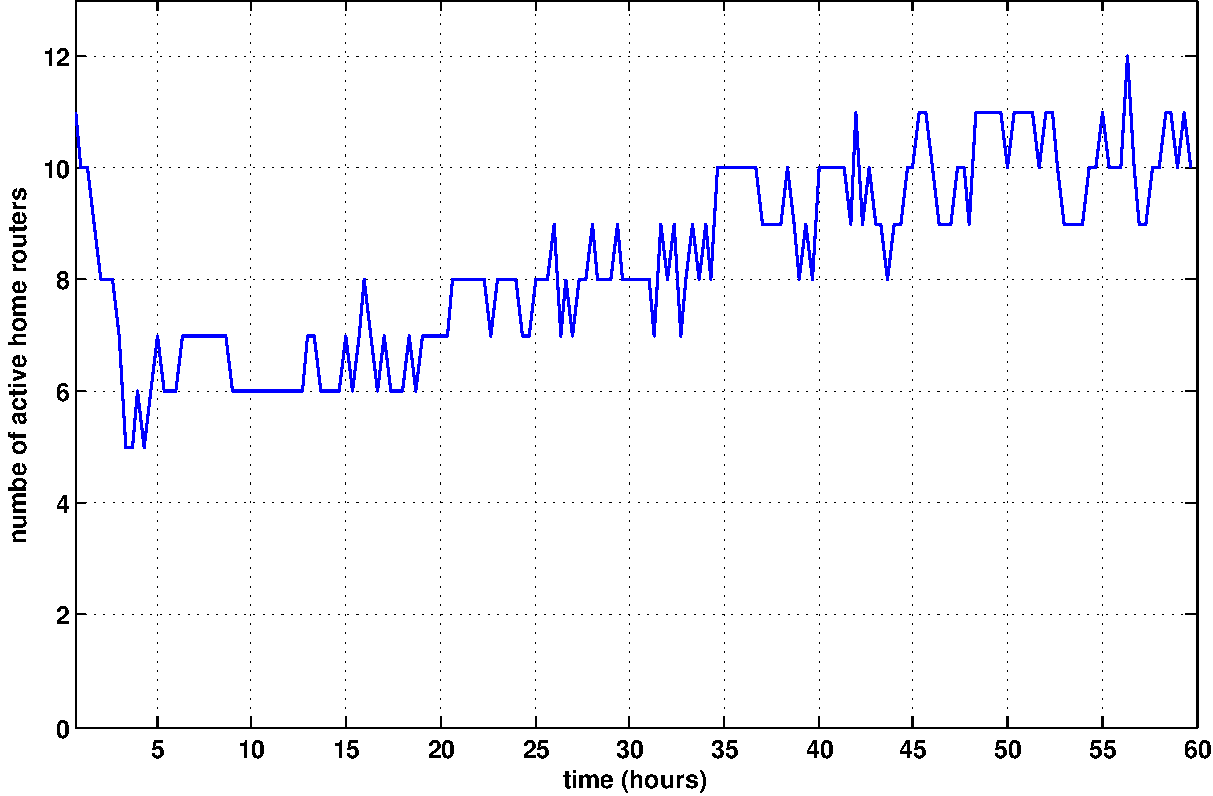
\includegraphics[width=1\linewidth]{results/on_routers.pdf}
\caption{Number of active home routers.}
\label{fig:active_routers}
\end{center}
\end{figure}

%To grant Internet access to the flows, the simulator implements two methods. The first method only give access to flows through the router at which they arrive given that there is enough internet access capacity. This method ignores the mesh network. On the other hand, the second method considers the mesh network by redirecting flows which does not fit in the local access routers to other routers through the mesh network. The router to which the flow is redirected are selected using worst-fit decreasing algorithm. The algorithm starts by sorting the flows to be redirected in non-decreasing order of their rates. Then, for each flow (starting with the flow with the highest rate), the algorithm selects the router with the highest available internet access capacity which fits the flow rate. The shortest path between the router is chosen based on the number of hops. The worst-fit decreasing algorithm is also used to redirect flows when a router goes OFF. This sustains as much as possible flows in the network and reduce disruption by the routers owners sharing policy.
%Furthermore, to show performance of the system under dynamic communication pattern, we consider flows with limited life time which arrive and leave the system at certain time point.

\begin{figure}[t]
\begin{center}
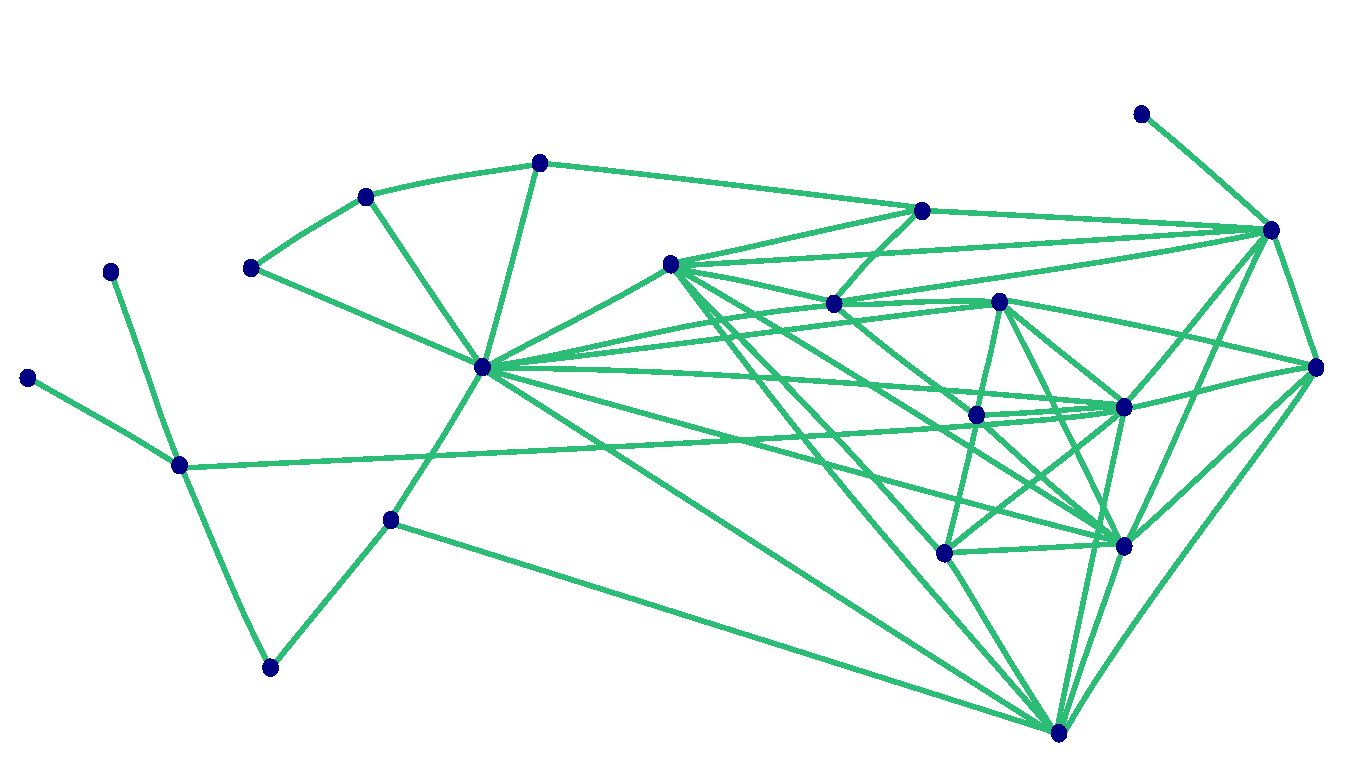
\includegraphics[width=1\linewidth]{topology.pdf}
\caption{Simulation WMN topology.}
\label{fig:topology}
\end{center}
\end{figure}

Guest user flows are granted Internet access either through local routers or by redirection to remote routers based on the algorithm presented in Section \ref{architecture:redirection}. Flows which cannot be accommodated are rejected. We evaluate the benefit of WMN in the context of crowd-shared Internet access using the total shared bandwidth utilization in all home routers as well as the accumulated serving rate. We define the accumulated serving rate $ASR(T)$ at time $T$ as:

\begin{equation}\label{1}
ASR(T)= \frac{\Sigma^T_t s^{finished}_{t}}{(\Sigma^T_t s^{finished}_{t} + \Sigma^T_t s^{rejected}_{t})},
\end{equation}
%
%${the accumulated acceptance rate =\displaystyle \frac{the\ total\ rates\ of\ flows\ finished\ up\ to\ t} {(the total rates of flows finished up to t + total rates of rejected flows up to t)}}$.
where $s^{finished}_{t}$ denotes the total sizes of the flows at time $t$ which are accepted (assigned Internet access) and successfully served without disruption due to router unavailability. $s^{rejected}_{t}$ denotes the total sizes of the flows at time $t$ which are rejected (not assigned Internet access).

Each simulation run comprises 60 hours at a time discretization of 20 minutes. For each scenario, we perform 20 simulation runs. We assume a homogeneous setting where each router has 16 Mbps ADSL downlink and set the shared bandwidth per router to 8 Mbps (i.e., in the periods that each router is active). We run our simulation with mesh link capacity of 200, 54 and 10 Mbps; this does not have any impact on the simulation results, since the bottleneck is the Internet access links. Our wireless link model does not consider the impact of interference and distance on the offered link bandwidth.

\subsection{Simulation Results}
\label{evaluation:results}

Initially, we measure the shared bandwidth utilization and serving rate with an arrival rate of 50 flows per minute over a 60-hour period. Fig. \ref{fig:utilization} illustrates a low utilization of the shared bandwidth without a WMN during the whole period, although there is high demand for Internet access by guest users attached to the various home networks. In contrast, a WMN allows to capitalize the unused capacity and accommodate a larger volume of guest user traffic. More precisely, according to Fig. \ref{fig:utilization} guest user traffic redirection through the WMN results in the full utilization of the shared bandwidth. Furthermore, crowd-shared WMNs can accommodate substantially larger volume of guest user traffic, as depicted in Fig. \ref{fig:acceptance}. This stems from the high utilization of the shared bandwidth.

\begin{figure}[t]
\begin{center}
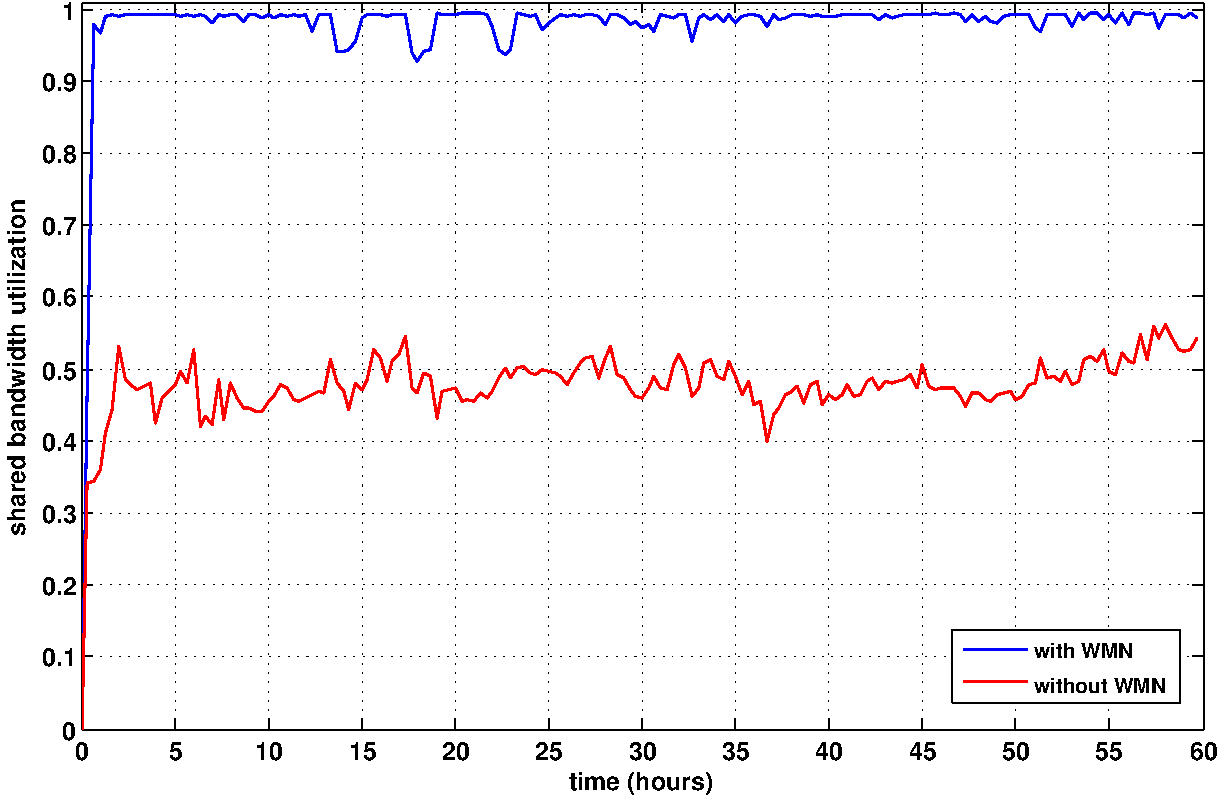
\includegraphics[width=1\linewidth]{results/utilization.pdf}
\caption{Shared bandwidth utilization.}
\label{fig:utilization}
\end{center}
\end{figure}

\begin{figure}[t]
\begin{center}
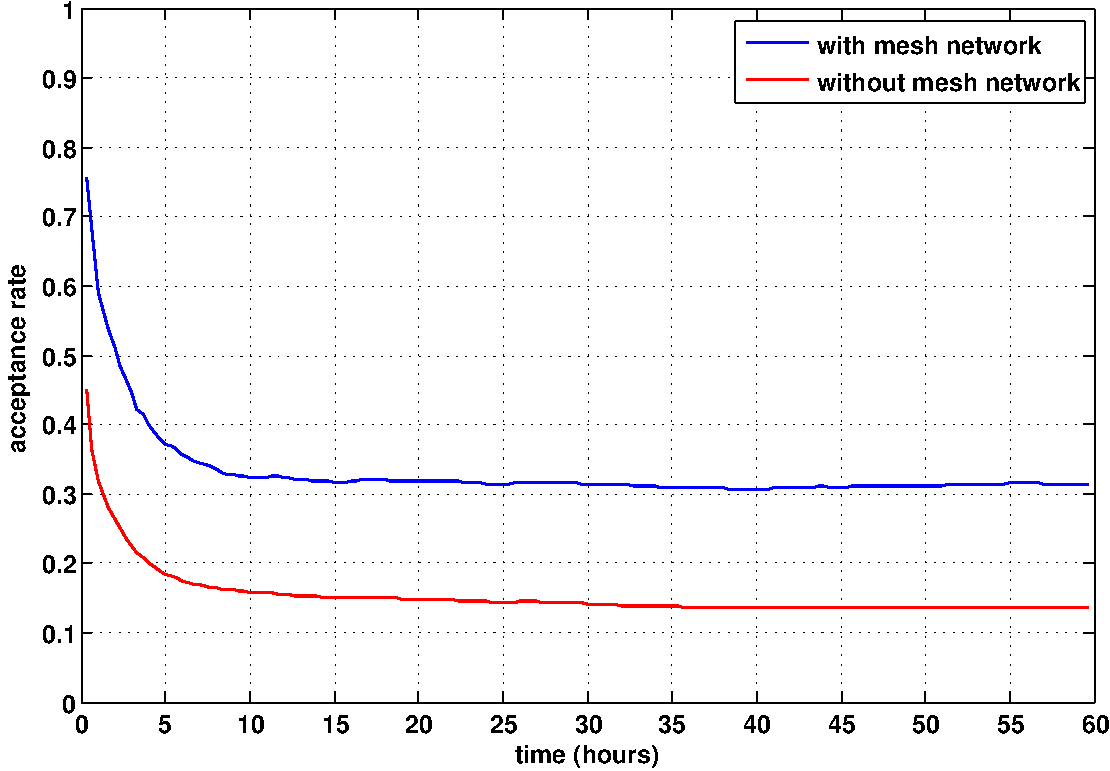
\includegraphics[width=1\linewidth]{results/acceptance_rate.pdf}
\caption{Accumulated serving rate.}
\label{fig:acceptance}
\end{center}
\end{figure}

We further measure the shared bandwidth utilization with a wide range of guest user traffic demands. In this respect, Fig. \ref{fig:utilization_arrival} illustrates the shared bandwidth utilization with diverse flow arrival rates, ranging from 10 to 100 flows per minute. Boxes show interquartile ranges and the median, with the whiskers showing the $5^{th}$ and $95^{th}$ percentiles. This simulation result corroborates the efficiency of the WMN for various traffic loads, as the shared bandwidth utilization always remains very high. Fig. \ref{fig:utilization_arrival} shows poor bandwidth utilization without a WMN, especially with low guest user traffic demand. In this particular case, the limitation of one point of Internet access for each guest user leads to wasting most of the shared bandwidth. Essentially, our simulation results show the significant benefit that a WMN can bring into crowd-shared networks, by effectively pooling resources across all home networks.

\begin{figure}[t]
\begin{center}
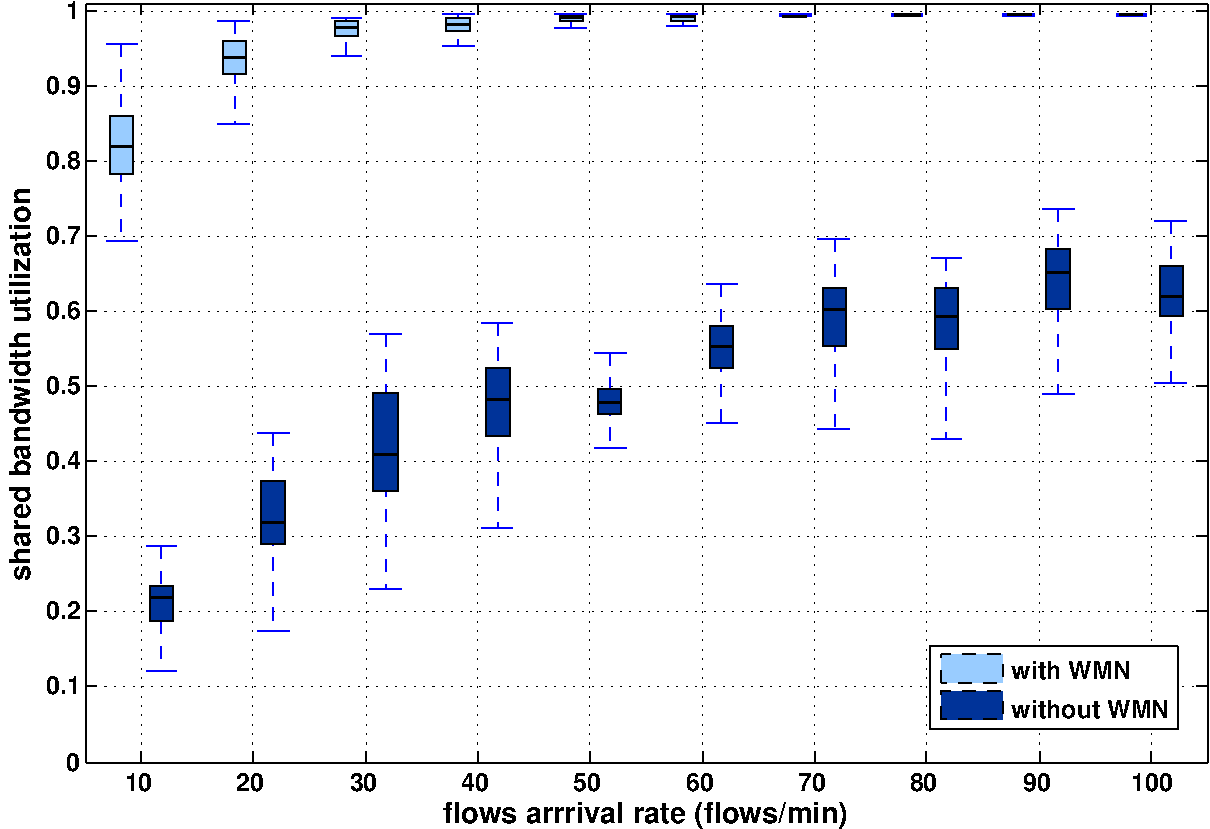
\includegraphics[width=1\linewidth]{results/boxplot2.pdf}
\caption{Shared bandwidth utilization vs. flow arrival rate.}
\label{fig:utilization_arrival}
\end{center}
\end{figure}

According to our simulations, redirected guest user traffic traverses up to 4 hops in the WMN. We further use a variant of our gateway and path assignment algorithm (briefly discussed in Section \ref{architecture:redirection}) which introduces a threshold in the number of hops between the home router and the assigned gateway. Fig. \ref{fig:hop_count} illustrates the shared bandwidth utilization for diverse hop-count threshold values ranging from 1 to 3, and without any limit in the hop count. Restricting the number of hops has a noticeable impact on bandwidth utilization, especially for a single hop, since Internet access is permitted only through one of the next-hop home routers. In essence, there is a trade-off between coverage extension (and thus effective bandwidth utilization) and latency. This may become more critical in large WMNs, where multi-hop wireless links can inflate latency.


\begin{figure}[t]
\begin{center}
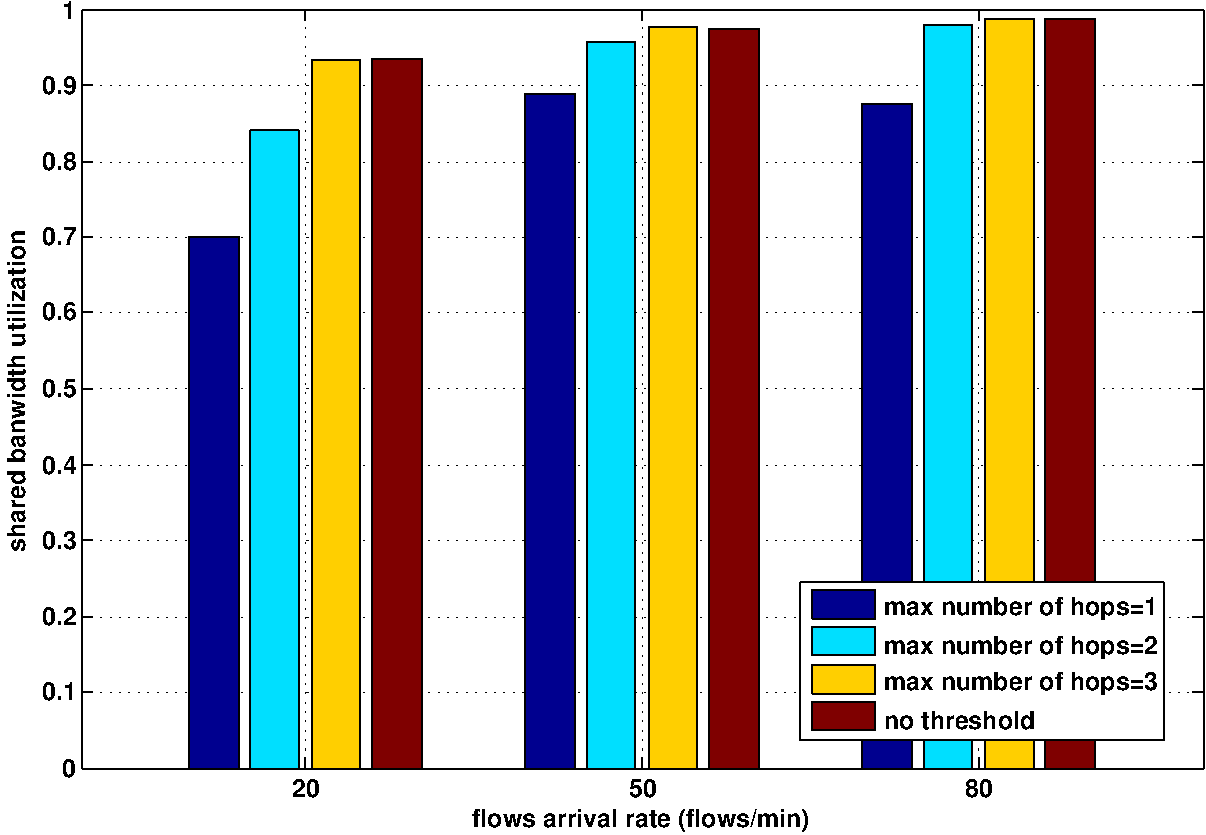
\includegraphics[width=1\linewidth]{results/hops_vs_BW.pdf}
\caption{Shared bandwidth utilization for diverse hop-count threshold values vs. flow arrival rate.}
\label{fig:hop_count}
\end{center}
\end{figure}

